\documentclass[ngerman,hyperref={pdfpagelabels=false}]{beamer}

% -----------------------------------------------------------------------------

\graphicspath{{images/}}

% -----------------------------------------------------------------------------

\usetheme{KIT}

\setbeamercovered{transparent}
%\setbeamertemplate{enumerate items}[ball]

\newenvironment<>{KITtestblock}[2][]
{\begin{KITcolblock}<#1>{#2}{KITblack15}{KITblack50}}
{\end{KITcolblock}}

\usepackage[ngerman,english]{babel}
\usepackage[utf8]{inputenc}
\usepackage[TS1,T1]{fontenc}
\usepackage{array}
\usepackage{multicol}
\usepackage[absolute,overlay]{textpos}
\usepackage{beamerKITdefs}

\pdfpageattr {/Group << /S /Transparency /I true /CS /DeviceRGB>>}	%required to prevent color shifting withd transparent images


\title{Algorithmen I - Tutorium 11}
\subtitle{Sebastian Schmidt -- \textit{isibboi@gmail.com}}

\author[Sebastian Schmidt]{Sebastian Schmidt}
\institute{Arbeitsgruppe Kryptographie und Sicherheit}

\TitleImage[width=\titleimagewd,height=\titleimageht]{titel}

\KITinstitute{Arbeitsgruppe Kryptographie und Sicherheit}
\KITfaculty{Fakult\"at f\"ur Informatik}

% -----------------------------------------------------------------------------

\begin{document}
\setlength\textheight{7cm} %required for correct vertical alignment, if [t] is not used as documentclass parameter


% title frame
\begin{frame}
  \maketitle
\end{frame}

\begin{frame}{Minimale Spannbäume}
Sei $G = (V, E)$ ein Graph.

\vspace{1em}
\emph{Schnitteigenschaft:}

Sei $S \subset E$ ein Schnitt in $G$.
Dann gehört eine Kante mit dem kleinsten Gewicht in $S$ zum MST.

\vspace{1em}
\emph{Kreiseigenschaft:}

Sei $K \subset E$ ein Kreis in $G$.
Dann gehört eine größte Kante auf $K$ nicht zum MST.

\pause
\vspace{1em}
Was ist der MST zum gegebenen Beispielgraphen? (Tafel)
\end{frame}

\begin{frame}{Jarník-Prim}
\vspace{-1.9em}
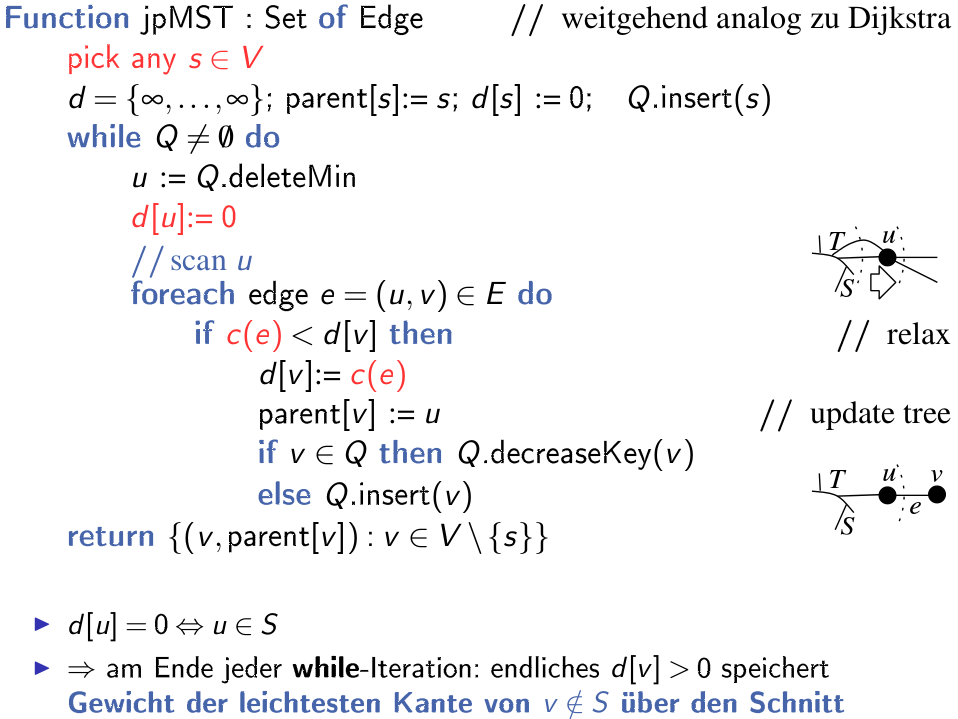
\includegraphics[width=0.9\textwidth]{jp}
\end{frame}

\begin{frame}{Kruskal}
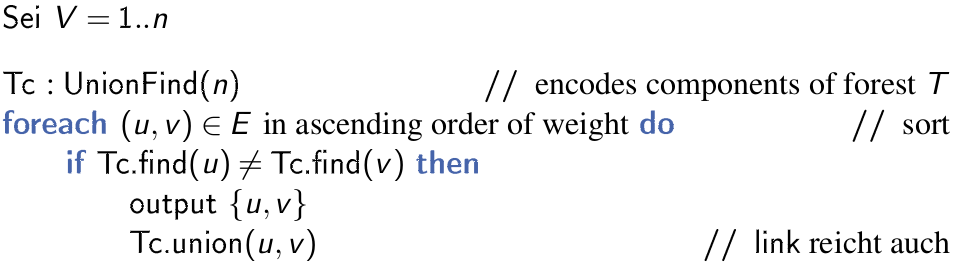
\includegraphics[width=\textwidth]{k}
\end{frame}

\begin{frame}
\centering
\vspace{-4em}
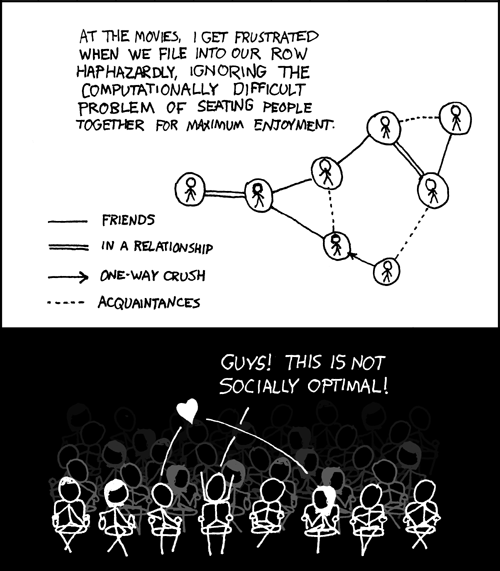
\includegraphics[width=0.66\textwidth]{movie_seating}
\end{frame}


\end{document}
